% Poche
\documentclass[paper=4.25in:6.87in,pagesize=pdftex,10pt,
               headinclude=on,footinclude=on]{scrbook}
\areaset[0.50in]{2.75in}{5.87in}

\title{Le témoignage que Jésus se rend à lui-même}
\author{Charles-\'Edouard Babut}

\usepackage{temoignage}

\newcommand{\isbn}{978-2-9539988-1-8}

\begin{document}

\frontmatter
\setlength{\parindent}{0em}
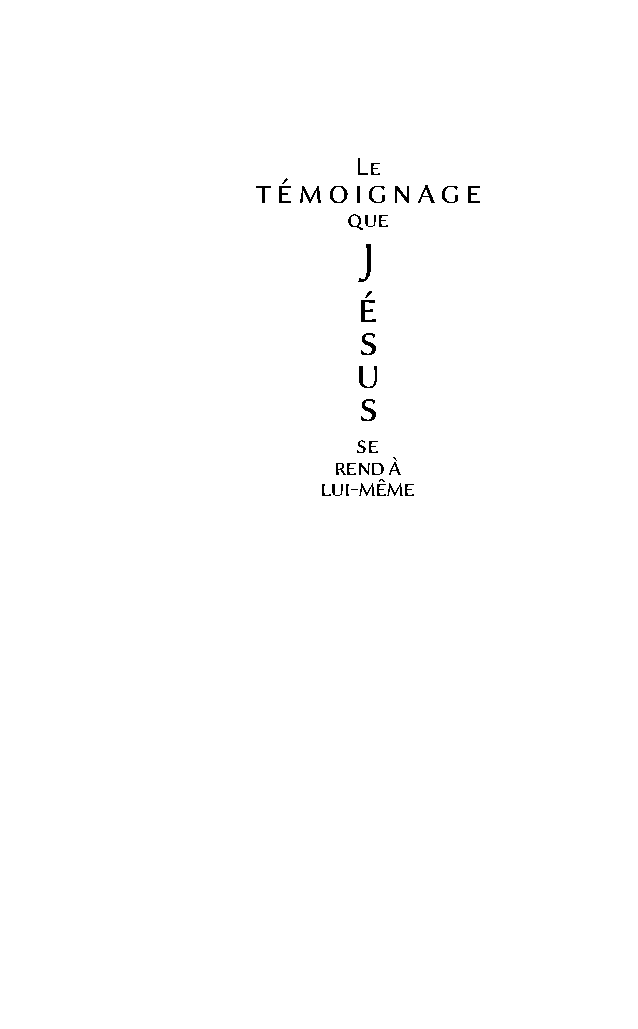
\includepdf{temoignage_fake_title}
\cleardoublepage
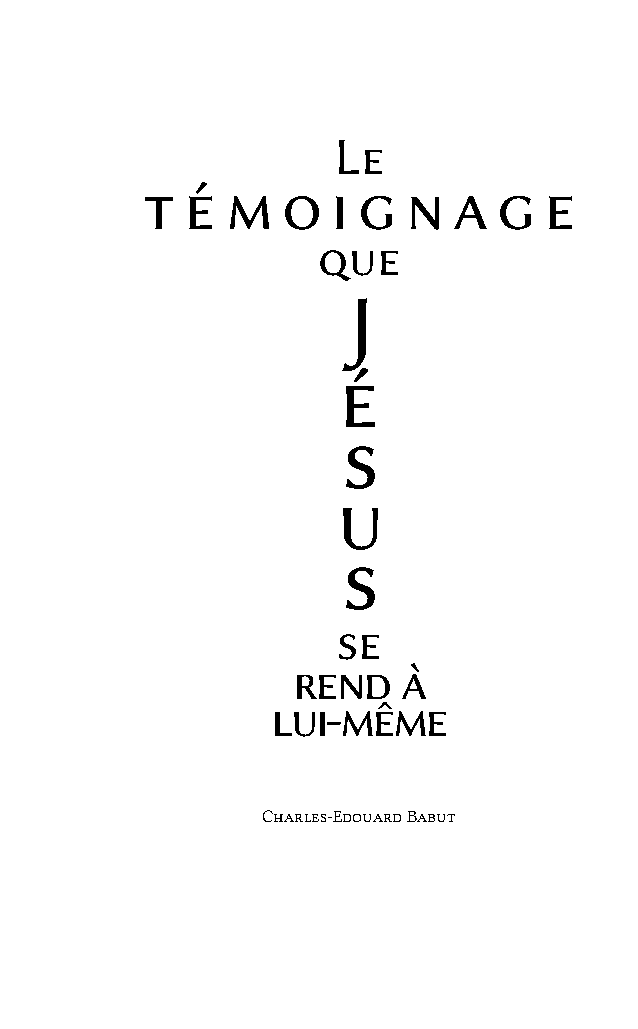
\includepdf{temoignage_title}
\pagestyle{empty}
% Copyright page
\newpage
\mbox{}
\vfill

{\scriptsize

{\bfseries Le témoignage que Jésus se rend à lui-même}

{\bfseries Certains droits réservés}

\ifluatex
  
\includegraphics[width=6em]{images/by-nc-nd_eu}
\fi

Cette \oe{}uvre est mise à disposition selon les termes de la \\
 Licence Creative Commons Paternité \\
 \ocadr Pas d'Utilisation Commerciale \\
 \ocadr Pas de Modification 2.0 France.

Le texte complet de cette licence est disponible sur \\
 \url{http://creativecommons.org/licenses/by-nc-nd/2.0/fr/}.

À Dieu soit la gloire!

}
\enlargethispage{\footskip}
\pagebreak




% Dedication page
\newpage
\mbox{}
\vfill


\begin{myverse}
{\itshape
Confie-toi en l'Éternel\\
 de tout ton cœur,\\
et ne t'appuie pas\\ sur ton intelligence.\\[5mm]
\Og{}Quoique je rende témoignage de moi-même, \\
 mon témoignage est véritable, \\
 car je sais d’où je suis venu et où je vais ; \\
 mais vous, vous ne savez d’où je viens, ni où je vais.\Fg{}
}
\myversereffont\bfseries\scshape \bibleverse{Jn}(8:14)
\end{myverse}
\vfill
\mbox{}
\newpage


\setlength{\parindent}{1em}

% Debug overfull boxes
\overfullrule=1mm
\tolerance=800

\mainmatter
\pagestyle{scrheadings}
\pagenumbering{arabic}
\addchap{Le témoignage\\ que Jésus se rend\\ à lui-même}

Mes frères\footnote{Sermon prêché le 5 juin 1872 dans le temple de l’Oratoire, à Paris, à l’occasion de l'ouverture du XXX\up{e} synode général de l'Église réformée de France.},

C’est le 10 janvier 1660 que se dispersa le dernier synode national des Églises réformées de France ; le dernier du moins qui ait été tenu avec l’autorisation des pouvoirs publics, le synode de Loudun. A peine réuni, il avait eu la douleur d’apprendre, de la bouche du commissaire royal, que Sa Majesté (Louis XIV) avait résolu « que l’on n’assemblerait plus de synodes nationaux que lorsqu’elle le jugerait expédient». Vainement le synode protesta de toutes ses forces, par l’organe de son modérateur, Jean Daillé, qui alla jusqu’à dire : « Il est entièrement impossible que notre religion puisse se conserver sans tenir de ces sortes d’assemblées.» S’il eût été sincère, le gouvernement aurait répondu qu’il partageait cette opinion, et que la destruction de la religion « prétendue réformée» était précisément son but.

Les synodes du Désert, si grands par leur fidélité, par leur courage, par leur sagesse, ne furent pas, dans la rigueur du terme, des synodes nationaux. Le dernier de ces synodes se réunit dans le bas Languedoc, en 1763 ; son acte le plus saillant fut un engagement solennel par lequel les députés s’obligèrent à l’unanimité à maintenir de tout leur pouvoir, dans les Églises, l’unité de foi, de culte, de morale et de discipline.

Demain, 6 juin 1872, l’Église réformée de France rentre en possession de son régime synodal, sous la protection du gouvernement de la République française, qui s’est montré aussi jaloux de respecter nos libertés, et même aussi empressé à nous les rendre, que le despotisme de Louis XIV était acharné à nous les ravir.

Gloire à Dieu, qui a eu compassion de notre Église, tout en l’éprouvant, et qui n’a pas permis qu’elle fondît tout entière dans le feu de la persécution la plus implacable, la plus systématique, la plus opiniâtre qui fut jamais ! Gloire à Dieu, qui la visite aujourd’hui dans sa miséricorde, et qui, en lui rendant l’institution qui est tout ensemble la garantie de son unité et la sauvegarde de ses libertés, l’appelle à entrer dans une ère nouvelle d’activité et de vie !

Et pourtant, avouons-le, mes frères : dans ce jour, dont la seule perspective eût fait bondir de joie le cœur de nos pères, des pensées de tristesse, d’inquiétude, ne sont étrangères à aucun membre du synode ; elles dominent chez quelques-uns. J’en dirai tout de suite la cause, attendu qu’il n’est ni bon, ni utile, ni possible de la dissimuler. Ce qui a fait la grandeur de notre Église, c’est sa foi. Cette foi, le premier de nos synodes, celui de 1559, à Paris, l’exprima d’un accord unanime dans une admirable confession qu’il écrivit en quelque sorte avec le sang des martyrs, au pied des échafauds et à la lueur des bûchers, et qu’on appela plus tard « la Confession de La Rochelle». A partir de ce jour, chaque nouveau synode national, au début de ses séances, lisait, sanctionnait, signait la confession de foi. Aujourd’hui nos Églises, privées depuis deux siècles de gouvernement central et régulier, n’ayant d’ailleurs ni pu ni voulu rester étrangères au mouvement de la pensée humaine durant ce long intervalle, ne sont plus unies dans la foi, comme elles l’étaient jadis. Étrange et cruelle situation ! Nous n’avons plus rien à craindre du gouvernement ni de la société qui nous entoure, mais nos divisions intérieures nous font plus de mal que la persécution elle-même n’a jamais pu nous en faire. Nous avons toute liberté pour affirmer, pour prêcher, dans une grande mesure pour propager nos croyances ; mais, comme Église, nous ne savons plus exactement ce que nous croyons. Membres du synode de 1872, que ferons-nous de cette question suprême, la question de la foi ? L’écarter par une fin de non-recevoir, n’est-ce pas décider et déclarer au monde que l’Église réformée n’est plus une Église, c’est-à-dire une société d’hommes attachés aux mêmes principes religieux, mais une association factice, un souvenir respectable, une expression historique, je ne veux pas dire un chapitre au budget ? Tenter de résoudre cette question, n’est-ce pas nous diviser ? n’est-ce pas provoquer un schisme ?

Mes frères, ne craignez pas que je me permette d’anticiper sur les résolutions du synode ou même sur ses délibérations. Je me souviens que c’est en qualité de prédicateur de l’Évangile que je suis dans cette chaire, et je veux porter votre attention et la mienne plus haut que le terrain ecclésiastique. La question qui nous divise : « Quelle est ou quelle doit être la base religieuse de notre Église ?» dépend évidemment de cette question plus générale : « Quel est le fondement même de la foi chrétienne ?» Car, en qualité de chrétiens protestants, nous voulons tous retenir le fondement ; mais lorsqu’il s’agit de bâtir ceci ou cela sur le fondement, nous réclamons pour nous-mêmes et nous accordons aux autres la liberté. Or, mes frères, à la question que je viens de formuler, je pense que nous serons tous d’accord pour répondre avec saint Paul : « Nul ne peut poser d’autre fondement que celui qui a été posé, à savoir, Jésus-Christ.» Mais peut-être n’apercevons-nous pas au premier abord toutes les conséquences de ce principe. La foi chrétienne est la foi en Jésus-Christ, c’est une proposition évidente par elle-même. Jésus-Christ est donc l’objet de la foi ; mais s’il en est l’objet, il en est aussi la raison et la règle ; autrement il n’en serait pas vraiment et souverainement l’objet. Le chrétien catholique romain croit en Jésus-Christ à cause de l’Église et conformément à ce que l’Église enseigne de lui : ce qui revient, dans la pratique, à mettre l’autorité de l’Église, c’est-à-dire aujourd’hui celle du pape, au-dessus de celle de Jésus-Christ. Le chrétien rationaliste croit en Jésus-Christ à cause de sa propre raison, et selon ce que sa raison admet ou conçoit : c’est-à-dire qu’en fait il met sa raison et sa conscience personnelles au-dessus de Jésus-Christ. Le chrétien évangélique, je veux dire le chrétien complet et conséquent dans sa foi, croit en Jésus-Christ à cause de Jésus-Christ et selon ce que Jésus-Christ a dit et pensé de lui-même. Le témoignage que Jésus-Christ a rendu de sa propre personne, est tout ensemble le dernier fondement et la règle suprême de sa foi. Le Seigneur Jésus, comme il le dit lui-même dans les paroles qui précèdent immédiatement notre texte, est la lumière du monde ; or, la lumière se prouve en se montrant et n’a pas besoin pour être aperçue d’une autre clarté que la sienne. C’est ce témoignage de Jésus-Christ, fondement inébranlable de la foi du chrétien et de la foi de l’Église, dont je me propose de montrer aujourd’hui la nature et la force. Un tel sujet, tout en nous élevant au-dessus de nos tristes débats ecclésiastiques, me paraît profondément actuel, dans le meilleur sens du mot ; il a de plus un autre avantage, inappréciable à mes yeux, celui de reléguer dans l’ombre la personne et les opinions particulières du prédicateur. Il m’en a coûté, croyez-le bien, d’accepter l’honneur immérité qui m’était offert et de m’adresser, dans une circonstance si solennelle, à une assemblée où j’aperçois en grand nombre mes supérieurs par l’intelligence et par la science, mes aînés dans la vie, dans le ministère et dans la foi. Pourtant j’ose vous dire comme Etienne : « Mes frères et mes pères, écoutez-moi»; car ce n’est pas pour les pensées d’un homme pécheur que je réclame votre attention, c’est pour Jésus-Christ lui-même vous parlant de Jésus-Christ.



% Do this automatically
\clearpage
% Needs improvement for title
\section{I}

\Og{} Quoique je rende témoignage de moi-même, mon témoignage est véritable, car je sais d’où je viens et où je vais.\Fg{} Quel est, mes frères, le témoignage auquel le Seigneur fait allusion dans ces paroles solennelles ? En d’autres termes, qu’est-ce que Jésus-Christ a dit de lui-même ? \ocadr{} Pour répondre d’une manière complète à cette question, pour reproduire intégralement le témoignage de Jésus touchant sa personne, il faudrait citer la moitié de ses discours ; pour le commenter, il faudrait écrire un livre, un livre qui, s’il allait au fond des choses, serait tout ensemble la meilleure exposition et la meilleure apologie de la vérité chrétienne. En raison des limites étroites qui nous sont assignées, nous ne pourrons qu’effleurer les sommets de notre sujet. Pour ne pas lasser votre attention, nous ne citerons pas toujours tout au long les paroles du Maître ; aussi bien vous sont-elles familières ; mais nous ne dirons rien qui ne soit appuyé sur des textes précis et positifs et nous nous appliquerons à rester en deçà de ce qu’ils affirment plutôt que de le dépasser.

Un premier fait s’impose à notre attention\frcolon{} Jésus-Christ est, dans tout le domaine de la Révélation, le seul envoyé de Dieu qui rende témoignage de lui-même. Les autres, comme il convient à des pécheurs chargés d’un si grand message, s’effacent devant la vérité qu’ils annoncent, se sentent petits, faibles, indignes en face de la mission qui leur est confiée. Paul, celui de tous qui, contraint par les circonstances, met le plus en avant sa personnalité, se défend absolument de toute prétention à se prêcher lui-même, et quand il apprend qu’un parti religieux se réclame de son nom, il s’indigne et s’écrie\frcolon{} \Og{} Avez-vous donc été baptisés au nom de Paul?\Fg{}\footverse{{ICo}(1:12-16)} Il en est tout autrement de Jésus. Son enseignement est, au moins en très grande partie, une révélation de sa personne. Il est même l’objet des doctrines qu’il prêche, des devoirs qu’il impose, des sentiments religieux qu’il inspire. Il veut qu’on croie en lui, qu’on s’attache à lui ; être persécuté pour son nom ou persécuté pour la justice, c’est la même chose\footverse{{Mt}(5:10)}; son nom ou sa personne se confond avec la religion, avec la vérité même\footverse{{Jn}(14:6)}. Il n’y a que deux explications possibles à un tel fait\frcolon{} ou bien Jésus est, pour dire le moins, beaucoup moins humble que ne le sont ses prédécesseurs ou ses disciples ; ou bien il y a entre eux et lui une différence vraiment essentielle.

Quelle est cette différence ? Ici, mes frères, nous n’osons pas imiter le vol d’aigle d’un saint Jean, qui d’un seul coup d’aile se transporte au plus haut des cieux et va chercher dans le sein de l’éternité et de la divinité même Celui dont il va raconter l’histoire. Il convient mieux aux besoins et aux habitudes de l’esprit moderne et aussi à la faiblesse de notre foi, de prendre la terre pour point de départ. Aussi bien, c’est ce que fit Jésus-Christ lui-même. Le nom qu’il affectionnait le plus est celui de Fils de l’homme, nom dont nous n’avons pas le temps de discuter le sens précis et d’indiquer les origines prophétiques, mais qui, pour tout esprit non prévenu, implique certainement ces deux choses\frcolon{} Jésus est homme, Jésus se sait et se sent, dans son humanité même, distinct du reste de l’humanité et supérieur à elle.
\quotebox{De même Christ, qui s’est offert une seule fois pour porter les péchés de beaucoup d’hommes, apparaîtra sans péché une seconde fois à ceux qui l’attendent pour leur salut.}{\ibibleverse{He}(9:28)}
Certes, Jésus est homme\frcolon{} chacune de ses paroles est une confession de son humanité et chacun de ses actes le révèle. Il est homme, on le sent à ses pleurs, à ses souffrances, à ses luttes, à ses tentations, à ses prières ; il est homme, d’une humanité réelle et complète, quant à son corps et quant à son âme ; \Og{} semblable en toutes choses à ses frères\Fg{}, dit un apôtre ; mais il ajoute\frcolon{} \Og{} sans péché\Fg{}.
Sans péché ! ces mots ne retranchent rien à l’humanité de Jésus, car, loin d’être un élément essentiel de la nature humaine, le péché est une infirmité, une dépravation de cette même nature ; mais ils suffisent à creuser un abîme entre Jésus et le reste des hommes, tels que l’expérience nous les fait connaître. Or, l’affirmation apostolique n’est, ici comme ailleurs, que l’écho de celle de Jésus lui-même.
Jésus se savait et s’est dit en mille manières pur de tout péché.
Je regarde ce fait comme le plus certain de l’histoire.
Je n’en appelle pas seulement à des déclarations expresses du Seigneur telles que celles-ci\frcolon{} \Og{} Qui de vous me convaincra de péché?\footverse{{Jn}(8:46)} \ocadr{} Le Père ne m’a point laissé seul, parce que je fais toujours ce qui lui est agréable.\footverse{{Jn}(8:29)} \ocadr{} Le Prince de ce monde vient, mais il n’a rien en moi.\Fg{}\footverse{{Jn}(14:30)}
\quotebox{\Og{} Ce ne sont pas ceux qui se portent bien qui ont besoin de médecin, mais les malades. Je ne suis pas venu appeler des justes, mais des pécheurs.\Fg{}}{\ibibleverse{Mc}(2:17)}

% This new paragraph was inserted to place the quote...
Tout l’ensemble de la vie et des discours de Jésus suppose absolument chez lui la conscience de sa sainteté parfaite, immaculée.
Il ne se met jamais sur le même rang que les pécheurs\frcolon{} ils sont les malades, lui le médecin.\footverse{{Mc}(2:17), \ibibleverse{Mt}(9:12), \ibibleverse{Lc}(5:31)}
Il y a un sentiment qu’il recommande à ses disciples comme étant pour eux le commencement et la condition de toute sainteté et dont il ne leur a jamais donné l’exemple, c’est le repentir. Essayez un moment de supposer qu’il ait eu sujet de répéter pour son propre compte ces mots de la prière qu’il nous a enseignée\frcolon{} \Og{} Père, pardonne-nous nos offenses\Fg{}\footverse{{Mt}(6:12), \ibibleverse{Lc}(11:4)}, vous n’ajoutez pas un trait à son image, vous la rendez grimaçante, monstrueuse, impossible ; vous anéantissez l’histoire évangélique tout entière. Chose merveilleuse ! Celui qui propose aux hommes la perfection absolue comme idéal et l’exacte imitation de Dieu comme loi, a la certitude intime qu’il observe lui-même cette loi et qu’il réalise cet idéal.

Jésus ne se sent pas seulement séparé des pécheurs par sa sainteté parfaite ; il se place vis-à-vis d’eux comme leur Maître, leur Législateur, leur Roi, leur Juge, leur Sauveur.
Plus grand qu’Abraham\footverse{{Jn}(8:58)}, que Moïse\footverse{{Mt}(19:8), \ibibleverse{Mc}(10:5)}, que David\footverse{{Mt}(22:44)}, que Salomon\footverse{{Mt}(12:42), \ibibleverse{Lc}(11:31)}, que le temple\footverse{{Mt}(12:6)}, que le sabbat\footverse{{Mt}(12:8), \ibibleverse{Mc}(2:27-28), \ibibleverse{Lc}(6:5)}, il est, je ne fais qu’abréger et résumer ses propres déclarations, il est celui qui accomplit la loi\footverse{{Mt}(5:17)}, celui que les prophètes ont désiré et attendu\footverse{{Mt}(13:17), \ibibleverse{Lc}(10:24)}, il est le propriétaire de ce champ qui est le monde\footverse{{Mt}(13:44)}, l’héritier de cette vigne qui est le royaume de Dieu\footverse{{Mt}(21:33-41), \ibibleverse{Mc}(12:1-9), \ibibleverse{Lc}(20:9-16)}, l’époux de cette élite sacrée de l’humanité qui formera son Église\footverse{{Mt}(22:1-14)}.
C’est lui qui, au dernier jour, rendra à chacun selon ses œuvres\footverse{{Mt}(16:27)}, séparera le blé de l’ivraie\footverse{{Mt}(13:24-30)}, les bons et les méchants\footverse{{Mt}(13:38)}; et ce qui déterminera la sentence des uns et des autres, ce sera d’avoir reçu ou rejeté la parole de Jésus\footverse{{Jn}(5:24)}, d’avoir aimé et secouru ce bon Maître dans la personne de ses disciples\footverse{{Mt}(25:40)}, ou de l’avoir méconnu et méprisé\footverse{{Mt}(25:41-43)}.
Il est le Sauveur de l’humanité perdue\footverse{{Jn}(12:47)}, le bon Berger\footverse{{Jn}(10:11,14)}, la Porte des brebis\footverse{{Jn}(10:7)}; il est le Médiateur entre Dieu et les hommes, \ocadr{} si le mot est de saint Paul\footverse{{ITim}(2:5)}, la pensée est partout dans les Évangiles.
Il est le chemin\frcolon{} d’abord le chemin de Dieu vers les hommes, et ensuite le chemin des hommes vers Dieu.
\quotebox{10}{Jésus lui dit: \Og{} Je suis le chemin, la vérité, et la vie. Nul ne vient au Père que par moi. \Fg{}}{\ibibleverse{Jn}(14:6)}

Quel que soit le bien que votre cœur réclame, Jésus vous convie à le chercher en lui ; \Og{} le trouver, c’est trouver toute chose\Fg{}. Vous avez soif de vérité\frcolon{} Jésus est la vérité, la lumière du monde ; le voir, c’est voir Dieu. Vous avez besoin de pardon\frcolon{} Jésus a le pouvoir de vous le donner, car il l’a acquis pour vous ; son sang coule sur la croix pour la rémission de vos offenses. Vous soupirez après le repos\frcolon{} Jésus le promet aux âmes travaillées qui viennent à lui ; il leur donne sa paix, et il ne donne pas comme le monde donne. Vous demandez le Saint-Esprit, c’est Jésus qui l’envoie ; vous êtes affamés et altérés de vie divine, Jésus donne l’eau vive, il est lui-même le Pain de vie ; il est le Cep dont la sève nourrit et féconde les sarments. Si quelqu’un a soif, qu’il vienne à lui et qu’il boive ! Assurément, Jésus veut conduire ses disciples à son Père et à leur Père, à son Dieu et à leur Dieu, mais il ajoute\frcolon{} \Og{} Nul ne vient au Père que par moi.\Fg{}

À ces déclarations si hautes de Jésus correspondent les sentiments qu’il réclame de ses disciples. Il exige d’eux une confiance absolue, une consécration sans réserve à son service, un amour ; sans bornes, devant lequel tout autre amour s’efface et se transforme presque en haine. Il veut qu’ils croient en lui comme en Dieu, qu’ils prient en son nom, qu’ils baptisent en son nom, qu’ils l’honorent comme ils honorent le Père. Encore une fois, quel contraste ne remarquons-nous pas à cet égard entre Jésus et tous les autres envoyés de Dieu ! Paul déchire ses vêtements quand les pauvres païens de Lystre veulent lui rendre les honneurs divins. Quand le voyant de l’Apocalypse veut se prosterner devant l’ange de la révélation, celui-ci le relève et lui dit\frcolon{} \Og{} Je ne suis que ton compagnon de service, adore Dieu.\Fg{} Jésus, lui, n’arrête et ne censure ni la foule qui crie\frcolon{} \Og{} Hosanna au fils de David !\Fg{} ni Simon-Pierre qui tombe à ses pieds, ni la femme pécheresse qui les embrasse, ni l’aveugle guéri qui l’adore, ni l’apôtre Thomas qui lui dit\frcolon{} \Og{} Mon Seigneur et mon Dieu !\Fg{} Certes, mes frères, dans toutes ces occasions, Jésus parle lorsqu’il se tait, et quand il accepte de tels hommages, c’est absolument comme s’il les réclamait lui-même.

Pour que Jésus prenne une telle attitude vis-à-vis des hommes, il faut qu’il soit et qu’il se sache dans un rapport unique avec Dieu. Il ne nous a pas laissés dans l’ignorance sur ce sublime sujet. Comme le nom qui définit ses rapports avec les hommes est celui de Fils de l’homme, le nom qui définit ses rapports avec Dieu est celui de Fils de Dieu. Jésus, sans doute, appelle ses disciples à devenir fils de Dieu, mais il se nomme \Og{} le Fils\Fg{} dans un sens excellent et unique, et parlant de Dieu, il ne dit pas \Og{} notre Père\Fg{}, il dit\frcolon{} \Og{} Mon Père et votre Père.\Fg{} Fils de Dieu, Jésus est subordonné à son Père et dépendant de lui ; il ne possède rien qu’il n’ait reçu du Père ; il fait les œuvres que le Père lui a montrées, il dit les paroles que le Père lui a dites ; il cherche la gloire du Père, non la sienne propre, il dit\frcolon{} \Og{} Le Père est plus grand que moi.\Fg{} Mais aussi le Père lui a tout dit, tout montré, tout donné. En qualité de Fils, il participe à toutes les perfections du Père, à sa science, à sa puissance, à sa vie ; la gloire de Dieu est sa gloire, les anges de Dieu sont ses anges, l’Esprit de Dieu est son esprit. À côté des passages où la subordination du Fils au Père est accentuée, se placent d’autres paroles où toute inégalité entre le Père et le Fils semble disparaître dans l’unité absolue, dans la réciprocité parfaite de l’amour\frcolon{} \Og{} Je suis dans le Père et le Père est en moi. Nul ne connaît le Fils que le Père et nul ne connaît le Père que le Fils. Tout ce qui est à moi est à toi ; et tout ce qui est à toi est à moi. Moi et le Père nous sommes un.\Fg{} \ocadr{} \Og{} Je sais d’où je viens et où je vais\Fg{}, dit Jésus dans mon texte. \ocadr{} D’où viens-tu, Seigneur ? \ocadr{} \Og{} Je suis d’en haut, je suis descendu du ciel ; avant qu’Abraham fût, je suis.\Fg{} \ocadr{} Où vas-tu ? \ocadr{} \Og{} Père, je vais à toi ; glorifie -moi de la gloire que j’ai eue auprès de toi, avant que le monde fût.\Fg{}

Tels sont quelques-uns des témoignages que Jésus a rendus touchant sa personne. On peut les résumer en peu de mots\frcolon{} Jésus se donne comme étant, dans le sens le plus élevé qu’il soit possible d’attacher à ses termes, le Saint de Dieu, le Sauveur du monde, le Médiateur entre Dieu et les hommes, le Fils de Dieu. Je m’arrête là. Je n’invoque aujourd’hui ni le témoignage de l’Église, ni celui des apôtres eux-mêmes. Je vous conduis tout droit et exclusivement à la source même de la vérité chrétienne, le cœur et la conscience de Jésus. Si vous recevez le témoignage de Jésus-Christ, vous pouvez être embarrassé pour en concilier les divers éléments et les réunir sans les altérer dans une conception tout ensemble précise, complète, harmonique ; mais enfin, vous êtes au clair sur le point essentiel, vous savez qui est Jésus-Christ, et ce qu’il est venu faire dans le monde. Si vous recevez le témoignage de Jésus-Christ, il peut y avoir encore à vos yeux plus d’un mystère non éclairci, plus d’une formule consacrée qui appelle une révision ; mais enfin, la grande question qui divise notre Église est résolue pour vous, et elle est résolue, je l’affirme hardiment, dans le sens de la doctrine évangélique et du christianisme surnaturel. Si vous recevez le témoignage de Jésus-Christ, vous avez besoin encore, et plus que jamais, que l’Esprit de Dieu vous explique et vous approprie la vérité écrite dans le livre, qu’il glorifie en vous votre Sauveur ; mais enfin vous n’êtes plus à la merci de tout vent de doctrine, vous avez trouvé le roc inébranlable sur lequel doit s’édifier votre foi comme la foi de l’Église.

Mais une crainte vous reste. Ce rocher lui-même ne serait-il pas miné à son tour par l’effort des siècles, par le flot montant de l’incrédulité ? En d’autres termes, le témoignage de Jésus-Christ est-il vraiment inattaquable ? N’y a-t-il rien qui doive nous troubler dans cette objection en apparence si plausible des pharisiens\frcolon{} \Og{} Tu rends témoignage de toi-même, ton témoignage n’est pas véritable\Fg{}? C’est ce qui nous reste à examiner.


%%II
Il y a deux moyens de récuser le témoignage de Jésus\frcolon{} le premier, c’est de le déclarer non authentique ; le second, c’est de le déclarer faux. Dans le premier cas, ce qui est attaqué, c’est la fidélité historique des Évangiles ; dans le second, c’est la véracité de Jésus, ou tout au moins sa compétence dans sa propre cause.

La première voie est la plus commode pour les adversaires, qui, en la suivant, ont l’avantage de paraître laisser de côté le Maître et ne s’en prendre qu’aux disciples. Le Christ divin, miraculeux, surnaturel, est, disent-ils, le fils de l’imagination et du pieux enthousiasme de l’Église. C’est surtout l’auteur du quatrième Évangile qui a fait le mal, en prêtant à Jésus ces affirmations exagérées sur sa personne dont on fait tant de bruit. Or, continuent-ils, cet auteur n’est pas l’apôtre Jean, mais un écrivain inconnu du II\up{e} siècle. \ocadr{} Ce n’est pas le lieu ni le moment, mes chers frères, d’énumérer les solides raisons qui me persuadent au contraire que le quatrième Évangile est bien de l’apôtre Jean. Un mot seulement à ceux d’entre vous qui ne sont pas théologiens. Sur les questions de cet ordre, ceux-ci ne sont pas toujours, quoi qu’on en dise, à la merci des savants. Ouvrez le quatrième Évangile, vous y verrez que l’auteur affirme catégoriquement qu’il fut témoin oculaire de la vie de Jésus, et trahit à chaque instant sa qualité d’apôtre\frcolon{} \Og{} Nous avons vu, dit-il, la gloire du Verbe devenu chair.\Fg{} Et ailleurs il s’écrie, à propos d’un détail de la crucifixion\frcolon{} \Og{} Celui qui l’a vu en a rendu témoignage, et son témoignage est véritable, et il sait qu’il dit vrai, afin que vous le croyiez.\Fg{} Cet auteur qui déclare avec tant d’insistance et de solennité qu’il a vu ce qu’il raconte, ce chrétien rempli du Saint-Esprit qui a écrit le quatrième Évangile, serait donc un faux témoin ? Ce serait un homme de la troisième ou quatrième génération chrétienne, qui aurait travaillé et réussi, avec une habileté incomparable, à se faire passer pour le disciple bien-aimé de Jésus ? \ocadr{} Telle est l’assertion à laquelle se condamnent eux-mêmes les adversaires de l’authenticité du quatrième Évangile. Je la soumets et la livre au verdict de vos consciences.

Mais enfin, supposons, tout éloignés que nous sommes de l’admettre, qu’on soit parvenu à écarter le quatrième Évangile, est-on débarrassé des témoignages que Jésus a rendus de lui-même ? Nullement. Ceux que contiennent les trois premiers Évangiles, s’ils sont un peu moins nombreux, ne sont pas moins explicites. C’est ici, je veux dire dans les trois premiers Évangiles, que Jésus parle de s’asseoir à la droite de son Père et de revenir pour juger le monde ; c’est ici qu’il se distingue, comme étant le Fils, de tous les prophètes qui l’ont précédé et qui ne sont que des serviteurs ; c’est ici qu’il établit que le Christ est le Seigneur de David en même temps que son Fils ; qu’il institue la sainte Cène, où il déclare, par le plus expressif des symboles, que sa chair déchirée et son sang répandu sont la vie des âmes, et que sa mort rédemptrice réconcilie les pécheurs avec Dieu ; c’est ici qu’en instituant le baptême, il place son nom entre celui du Père et celui du Saint-Esprit ; c’est ici que se trouvent des paroles telles que celle-ci.\frcolon{} \Og{} Toute puissance m’a été donnée dans les cieux et sur la terre\Fg{}, et celle-ci\frcolon{} \Og{} Je suis avec vous tous les jours jusqu’à la fin du monde\Fg{}; et celle-ci surtout, qui ne le cède en sublimité à aucune des déclarations contenues dans le quatrième Évangile\frcolon{} \Og{} Toutes choses m’ont été remises par le Père, et nul ne connaît le Fils que le Père, et nul ne connaît le Père que le Fils, et celui à qui le Fils l’aura voulu révéler.\Fg{} Il n’est presque pas un seul article du témoignage de Jésus touchant sa personne, tel qu’il a été exposé tout à l’heure, qui ne soit appuyé sur les trois premiers Évangiles aussi bien que sur le quatrième. Non moins frappants que ces témoignages directs sont les témoignages indirects, involontaires en quelque sorte, tels que celui-ci par exemple. Les apôtres disent à Jésus\frcolon{} \Og{} Augmente-nous la foi\Fg{}, et Jésus accepte cette prière, qui lui suppose le pouvoir tout divin d’agir directement et intérieurement sur les cœurs par son esprit. Et pourquoi non ? Jésus ne dit-il pas aussi à ses apôtres, dans le même Évangile, celui de saint Luc\frcolon{} \Og{} Je vous donnerai une bouche et une sagesse, à laquelle vos adversaires ne pourront résister\Fg{}? Si l’on ne veut pas que Jésus-Christ ait cru à sa propre divinité, il faudra rayer tous ces passages. Ce travail de mutilation arbitraire ne s’arrêtera pas là. Il n’est pas une seule portion de l’Évangile qu’il laisse entière\frcolon{} ni le Sermon sur la montagne, car Jésus s’y déclare le juge des hommes ; ni les paraboles, car il en est plusieurs qui expriment la même pensée ; ni le récit de la Passion, car, sans rappeler encore l’institution de la sainte Cène qui l’inaugure et qui l’explique, on y voit Jésus sur la croix ouvrir à un mourant, par sa parole royale, la porte du paradis. Comme la moindre parcelle d’un organisme vivant est organisée, ainsi, si faible que soit le résidu de paroles et de faits que laisse subsister une critique aveuglée par des préjugés hostiles à la foi, on y verra encore percer, par quelque endroit la conscience inébranlable qu’avait Jésus de la grandeur unique et divine de sa personne. Cette conscience divine de Jésus n’est pas une superfétation, un ornement qu’on puisse arracher de l’Évangile, elle en est le centre ; elle est l’âme des discours du Maître et la clef de son histoire ; elle produit et explique tout le reste\frcolon{} rôle messianique, miracles, doctrine, haine du monde, mort sanglante de Jésus ; et, sans elle, rien ne s’explique, tout est confus, contradictoire, impossible. Cependant, quand vous aurez réussi à construire, tant bien que mal, une vie de Jésus, après en avoir ôté la pierre angulaire, ce ne sera pas tout ; il restera à rendre compte de l’existence et de la foi de l’Église, ainsi que du reste du Nouveau Testament ; il faudra nous montrer comment les apôtres ont pu être tout à la fois assez inintelligents pour comprendre si mal leur maître, et assez ingénieux pour lui prêter des discours si profonds et si sublimes ; comment Paul, si bien placé pour être informé, et d’un esprit si lucide, a pu s’éprendre à son tour de cette étrange chimère, et mettre à la place du doux, rabbin de Nazareth, le Christ démontré Fils de Dieu avec puissance par sa résurrection d’entre les morts !… On a reculé, mes frères, devant tant d’impossibilités ; les plus hardis critiques, après avoir retranché tout ce qu’ils ont pu des témoignages de Jésus touchant sa personne, se sont aperçus qu’ils avaient gagné fort peu de chose, et, sans exception, ils ont fini par avouer que Jésus a en tout cas pensé et dit de lui-même des choses surprenantes, surnaturelles, incroyables par conséquent à leur sens, et qu’ils attribuent à ce qu’ils appellent ses \emph{illusions messianiques}.

Nous voici donc ramenés à la seconde hypothèse. Les pharisiens auraient raison ; le témoignage que Jésus aurait réellement rendu de lui-même ne serait pas véritable.

Examinons cette dernière supposition avec autant de brièveté et aussi avec autant de sang-froid que nous le pourrons.

Jésus donc, on l’accorde maintenant, a cru être sans péché ; il s’est considéré comme un personnage surnaturel ; il a pris la position de médiateur entre Dieu et les hommes ; il a prétendu avoir sur l’âme humaine des droits absolus et divins ; mais on ajoute qu’en tout cela il s’est trompé. – Ce qui rend cette opinion insoutenable et contradictoire, c’est que ceux qui la professent ne se défendent pas, et dans l’occasion, se vantent, au contraire, d’éprouver beaucoup de respect et d’admiration pour Jésus. Ils ne font pas difficulté de reconnaître qu’il est et restera toujours le premier des hommes, le plus sublime des croyants et des révélateurs. Ils l’appellent quelquefois leur Maître. Ils ne peuvent faire moins, considérant qu’il est d’évidence historique que Jésus a apporté au monde et mis dans le cœur des hommes une nouvelle connaissance, la connaissance du Père céleste ; une nouvelle espérance, l’espérance de la vie éternelle ; une nouvelle passion, la passion de la sainteté. En conséquence, sans pouvoir admettre que Jésus ait été exempt de faute et d’erreur, les critiques dont je parle voudraient et devraient tout au moins ne lui attribuer que de légères erreurs et d’excusables fautes. Mais c’est là précisément ce qui est impossible. Quoi ! se croire parfaitement saint, pur de toute souillure, quand, après tout, l’on est pécheur, ce serait une erreur excusable ? Mais ce serait au contraire le comble du pharisaïsme ! Et vous osez imputer cela à Jésus, le censeur impitoyable des pharisiens ! Ne savez-vous pas que, plus une conscience est pure, plus les moindres infractions au devoir s’y trahissent et s’y manifestent comme autant de taches sombres sur un fond brillant ? En vertu de cette loi, si Jésus avait été seulement le moins pécheur des hommes, il en aurait été le plus repentant. Or, voici qu’au contraire il se déclare certain de l’entière approbation de son Père, il se met à part du reste des hommes en leur disant\frcolon{} \Og{} Vous qui êtes mauvais !\Fg{} Il s’attribue le droit de les juger et le pouvoir de les sauver ! Certes, si de telles prétentions ne sont pas l’expression de la vérité même, elles sont le délire de l’orgueil. – Quoi encore ! s’arroger le rôle de médiateur entre Dieu et ses semblables, faire de sa propre personne l’objet de la foi, de l’amour suprême, de la religion du genre humain, s’asseoir sur le trône de Dieu, voulant se faire passer pour un Dieu, tout cela serait de la part de Jésus une regrettable, mais pardonnable illusion ! Mais ne vous rappelez-vous pas que les expressions mêmes que je viens d’employer sont celles par lesquelles l’apôtre Paul désigne l’Antichrist ? Blasphème ou folie, l’un au moins de ces deux mots suffirait seul à caractériser cette entreprise sacrilège. Étrange extrémité que celle où sont réduits ceux qui, tout en reconnaissant à quelque degré l’excellence morale de Jésus et la grandeur de son œuvre, refusent d’ajouter foi au témoignage qu’il rend de sa personne ! Leur Jésus est, tout à la fois, le plus saint et le plus coupable, le plus sage et le plus insensé des hommes, le Christ et l’Antichrist, le révélateur du Père et l’usurpateur de ses droits, le bienfaiteur et le séducteur du genre humain ! Qu’est-ce qu’un tel tissu de contradictions, sinon une évidente confirmation de la parole de mon texte, une justification éclatante de ce défi jeté par Jésus à ses adversaires de tous les temps\frcolon{} \Og{} Vous ne savez d’où je viens ni où je vais.\Fg{} Non, vous ne le savez pas, ô sages de ce monde, et vous ne le saurez jamais, tant que vous resterez étrangers à la sagesse de la foi ! Jésus vous est une obscure énigme, une éternelle et importune question, que vous ne pouvez ni écarter, ni résoudre. Son souvenir vous obsède ; il dérange vos théories ; il vous impose toujours de nouvelles recherches ; par là du moins vous êtes contraints de lui rendre hommage. Mais comme, pour savoir qui est Jésus, vous ne voulez pas vous en rapporter à Jésus lui-même, vous ne pouvez manquer de vous égarer. Vous vous mettez l’esprit à la gêne pour imaginer un Jésus qui ne dépasse pas de trop haut la stature des autres hommes ; mais vos créations fantastiques, semblables aux assertions des faux témoins soudoyés par Caïphe, ne s’accordent pas mieux avec elles-mêmes qu’avec la réalité ; elles ne satisfont pas plus la science que la foi, et après avoir excité un moment la curiosité publique, elles tombent dans un juste décri. Mieux vaudrait un simple aveu d’ignorance\frcolon{} Vous ne savez d’où il vient ni où il va. Mais ce que vous ignorez, Jésus le sait ; il le sait, lui seul. Qu’y a-t-il là d’étonnant ? \Og{} Nu ne sait ce qui est dans l’homme, dit saint Paul, excepté l’esprit de l’homme qui est en lui\Fg{}; ainsi nul ne sait ce qui est en Jésus, si ce n’est Jésus. À la vérité, un homme nous est suspect, pour l’ordinaire, quand il rend témoignage de lui-même ; mais pour quel motif ? parce qu’il peut aisément être aveuglé par l’amour-propre, l’intérêt, la passion ; pouvez-vous, de bonne foi, élever de tels soupçons contre Jésus ? Ne voyez-vous pas tout ce que d’une part la sainte vie et la sainte mort de Jésus, et d’autre part, l’œuvre incomparable qu’il a accomplie, ajoutent à la force de son témoignage ? Celui qui a contemplé Dieu dans le miroir de son âme pure et qui l’a révélé au monde, a-t-il pu s’abuser si étrangement sur lui-même et sur ses vrais rapports avec Dieu ? Ne discernez-vous pas, dans toutes ses paroles, et tout spécialement dans le témoignage qu’il rend de lui-même, cet accent de certitude tranquille et absolue, de souveraine autorité, qui jadis étonnait les multitudes ? Rejeter ce témoignage, c’est démentir le Père avec le Fils, l’histoire avec la révélation, le cri de la conscience humaine avec la voix de Dieu ; c’est se condamner logiquement à n’avoir plus d’autre croyance et d’autre sagesse que celle qui est résumée dans ce mot amer ou frivole de Pilate\frcolon{} \Og{} Qu’est-ce que la vérité ?\Fg{}

Mes frères, j’ai placé devant vous dans ses véritables termes la question de la foi et de l’incrédulité. Je vous ai mis en face de Jésus-Christ et de sa parole. Ne vous en rapportez pas à moi ; vérifiez les citations ; relisez les quatre Evangiles ; voyez si le témoignage de Jésus n’est pas tel que je vous l’ai présenté, et plus complet encore. Puis, si vous êtes encore de ceux qui doutent, pesez la valeur de ce témoignage ; choisissez, car il n’y a pas de milieu, entre l’assertion de Jésus\frcolon{} \Og{} Mon témoignage est véritable\Fg{}, et celle des pharisiens\frcolon{} \Og{} Ton témoignage n’est pas véritable.\Fg{} Le choix est sérieux et de grande conséquence. Car celui qui dit de lui-même de si grandes choses a dit aussi\frcolon{} \Og{} Celui qui croit en moi a la vie éternelle ; si vous ne croyez pas ce que je suis, vous mourrez dans vos péchés.\Fg{} Le choix est pressant, car la vie s’écoule ; vous ne pouvez pas demeurer dans l’incertitude ; vous ne devez pas du moins y demeurer volontairement un seul jour. Comme l’a dit le poète, il faut croire ou nier. Si vous arrivez à penser avec nous qu’en présence d’un témoignage comme celui de Jésus, la négation est véritablement impossible à une conscience droite, vous n’aurez plus de refuge que dans la foi. Et vous qui êtes déjà dans la foi, affermissez-vous dans cette foi sainte et bienheureuse en considérant combien le fondement en est solide, combien la source en est haute et pure. Ce fondement, cette source, c’est, ne nous lassons pas de le répéter, la conscience de Jésus lui-même, sa lumineuse et inaltérable conscience de Fils de Dieu…. Pourquoi donc nous laisserions-nous encore ébranler, soit par la contradiction du siècle, soit par les hésitations de notre pensée et les défaillances de nos cœurs ? Quand notre foi chancelle, retrempons-la dans sa source ; quand nos âmes se troublent, qu’elles s’approchent de l’âme de Jésus en méditant sa parole, et ce divin contact leur rendra la santé et la force. Nous ignorons, mais Jésus sait ; ailleurs, les motifs de doute, les causes d’erreur abondent, mais le témoignage de Jésus est véritable, que dis-je ? il est la vérité même ; or, ni le temps, ni le nombre, ni le talent, ni rien enfin en nous ou hors de nous, ne prévaudra contre la vérité.

Enfin, souvenons-nous, il faut y revenir en terminant, que ce fondement de la foi du chrétien est aussi le fondement de la foi de l’Église. Cela s’entend de soi ; car la vie de l’Église diffère en étendue, mais non en nature, de la vie du chrétien ; fait individuel ou collectif, le christianisme est toujours le même dans son essence. On a souvent dit que l’Église protestante reposait sur deux principes\frcolon{} un principe \emph{formel}, l’autorité des saintes Écritures en matière religieuse ; un principe \emph{matériel}, la justification par la foi. Nous estimons cette appréciation exacte et nous retenons pleinement ces deux principes. Toutefois, en creusant encore plus avant, nous croyons découvrir sous ce double fondement un fondement unique, Jésus-Christ\frcolon{} Jésus-Christ, la vie de nos âmes, le remède de nos maux, l’espoir de notre éternité ; Jésus-Christ notre seul Sauveur, car nos œuvres ne peuvent rien ajouter à sa justice parfaite ; Jésus-Christ notre seul maître, car les prophètes dont il a accompli et sanctionné les paroles, les apôtres qu’il a choisis et remplis de son Esprit, doivent essentiellement à Jésus-Christ l’autorité que nous leur attribuons. Voilà le véritable rocher sur lequel l’Église chrétienne est bâtie. Nous déplorons de toutes nos forces qu’une grande partie de cette Église superpose et, dans une grande mesure, substitue à ce fondement que Dieu lui-même a posé, je ne sais quel fondement vermoulu, je ne sais quelle infaillibilité de commande et d’invention humaine, décernée à un homme pécheur par des hommes pécheurs, et contre cette erreur impie, nous retrouvons au fond de nos consciences toute l’énergie des protestations du xvie siècle ! \ocadr{} Mais aussi nous n’appellerions pas chrétienne une Église qui n’aurait d’autre fondement que le libre examen. Le libre examen, droit et devoir pour tous en toute matière, particulièrement en matière religieuse, n’est pas même une philosophie, mais seulement la condition de toute philosophie ; combien moins est-il une religion ! Nous n’appellerions pas non plus chrétienne une Eglise qui mettrait à sa base, non pas le Christ éternel et vrai, le Christ des saintes Écritures, des apôtres et avant tout de Jésus lui-même, mais un Christ quelconque, le Christ qu’il plaît à chacun d’imaginer ou de concevoir, un Christ que ses prétendus disciples ont commencé par passer au crible de leur étroite raison, un Christ dépouillé de tout ce qui dépasse notre nature corrompue et dénaturée ; un Christ qui ne serait plus qu’un nom sans signification précise, un drapeau incolore, un ornement presque superflu de la religion et de la morale naturelles, une consécration mensongère prêtée à des doctrines toutes différentes de celles \ocadr{} et quelquefois contraires à celles \fcadr{} que le vrai Christ a prêchées et qu’il a scellées de son sang…

Mes bien-aimés frères, il faut qu’en terminant je dise toute ma pensée, dussé-je paraître m’écarter de l’intention que j’ai annoncée de n’anticiper en rien sur les délibérations du synode. J’avertis seulement que je ne parle qu’en mon propre nom, \ocadr{} je veux dire au nom des intérêts et des devoirs de l’Église, tels qu’il m’est donné de les comprendre, \fcadr{} et que mes paroles n’engagent que moi-même. Nous sommes jaloux des droits de la vérité, et des droits de la liberté aussi. Nous nous sentons profondément uni à nos pères par le fond de la foi ; nous croyons qu’il s’agit de prolonger avec intelligence leur tradition religieuse plutôt que de l’abandonner et de la renverser ; mais nous ne prétendons pas imposer comme un joug à nos frères ni à nous-même la lettre de leurs symboles, et si tel d’entre nous s’en écarte jusqu’ici, et tel autre jusque-là, nous ne pensons pas qu’il y ait dans cette divergence matière à séparation ou à schisme. Nous vénérons bien plus encore les saintes Écritures ; à nos yeux, l’enseignement religieux qu’elles contiennent est divin dans sa source et dans sa substance ; toutefois nous admettons que si le fond est divin, la forme est humaine à bien des égards ; si l’un de nous conçoit un peu autrement que tel autre le rapport de l’humain et du divin dans l’Écriture sainte ; s’il définit un peu autrement le mode et le degré de l’inspiration prophétique ou apostolique, nous ne pensons pas qu’il y ait là matière à séparation et à schisme. Mais nous ne comprenons pas comment ceux qui, de tout leur cœur, reconnaissent Jésus-Christ, c’est-à-dire, répétons-le, le Christ des apôtres et de Jésus lui-même, pour leur Maître et leur Seigneur, et ceux qui au fond n’ont d’autre règle de foi que leur sentiment individuel, pourraient être au même titre membres et docteurs d’une même Église. Les uns sont placés sur le terrain de la religion révélée, les autres sur celui de la philosophie. Nous ne jetons pas l’anathème à qui que ce soit, mais il faut absolument que nous rendions gloire à notre Seigneur et Sauveur. Il faut absolument qu’en face de notre patrie malade, mutilée, sur qui tous les médecins veulent essayer leur art et qui connaît si peu le véritable ; en face de ce siècle dévoyé, tourmenté, étourdi par les voix discordantes de la sagesse humaine, nous confessions que le témoignage de Jésus est la vérité et que la vérité n’est point ailleurs. Il faut absolument qu’à l’Église romaine et à son pape infaillible, nous opposions quelque chose de mieux que la souveraineté faillible du jugement individuel ; il faut que nous proclamions, nous aussi, notre Chef et notre Roi, Jésus-Christ, dans toute l’autorité de sa parole, dans toute l’efficacité de sa grâce et de sa rédemption, dans toute la majesté de sa personne divine et humaine. Si quelques-uns seulement, ce qu’à Dieu ne plaise, s’accordaient dans cette pensée… eh bien ! ces quelques-uns seraient contraints, la douleur dans l’âme, je ne sais par quelle voie, de former un groupe distinct autour de leur divin Chef ; et quel que fût leur nombre, majorité ou minorité, unis à l’État ou séparés de l’État, ils garderaient ou emporteraient avec eux tout le passé et tout l’avenir de l’Église réformée de France. Mais nous espérons de meilleures choses de la fidélité de notre Dieu ; nous espérons que l’Esprit de Dieu, que nous avons invoqué ce soir et que nous demandons à tous les fidèles d’invoquer chaque jour avec nous sur les délibérations du synode, dissipera bien des obscurités, fléchira bien des résistances. Nous espérons que notre Église, l’Église des martyrs, mise en demeure, après un si long silence, de dire ce qu’elle croit, voudra s’associer, non pas dans un esprit de dogmatisme sec et stérile, non pas avec les sous-entendus et les réticences d’une demi-foi, qui ne concède les mots que pour disputer sur les choses, mais avec l’élan d’une piété et d’une adoration véritables, à l’antique confession de Simon Pierre\frcolon{} \Og{} Seigneur, à qui irions-nous qu’à toi ? Tu as les paroles de la vie éternelle…. Nous avons cru et nous avons connu que tu es le Christ, le Fils du Dieu vivant. \Fg{}

Amen.     



\backmatter
\chindex

\ifluatex
%  \pagestyle{empty}
%  % Depot legal
\cleardoublepage
\mbox{}
\vfill

{\scriptsize
\begin{center}
Achevé d'imprimer au 1\up{er} trimestre 2015 \\
%Dépôt légal\frcolon{} 3\up{e} trimestre 2013
\end{center}
}
\enlargethispage{\footskip}




%  \clearpage
  \mbox{}
\fi


\end{document}





% Notes
% 1
% Jean 15.30.
% 2
% 1 Jean 1.8,10.
% 3
% Proverbes 20.9.
% 4
% Psaume 143.2.
% 5
% Luc 1.6,20.
% 6
% Matthieu 5.8.
% 7
% Luc 6.20.
% 8
% Matthieu 6.12.
% 9
% Psaume 130.4.
% 10
% Jérémie 13.23
% 11
% Ézéchiel 18.31
% 12
% Jacques 4.8
% 13
% 2 Corinthiens 5.17.
% 14
% Matthieu 9.29.
% 15
% Ésaïe 45.19.
% 16
% Zaccharie 13.1
% 17
% Sermon prêché le 5 juin 1872 dans le temple de l’Oratoire, à Paris, à l’occasion de l’ouverture du
% xxx
% e synode général de l’Église réformée de France
